% Параметры компиляции

\documentclass[a4document]{article}

\usepackage[utf8x]{inputenc}
\usepackage[english,russian]{babel}
\usepackage{cmap}

\thispagestyle{empty} 



\usepackage[14pt]{extsizes}
\usepackage[left=2cm,right=2cm,
    top=2cm,bottom=2cm]{geometry}
\usepackage[unicode, pdftex]{hyperref}
\usepackage{graphicx}
\usepackage{subcaption}



\begin{document}


% Титульный лист
{
\centering{
Министерство образования и науки Российской Федерации \\
Федеральное государственное автономное образовательное \\
учреждение высшего профессионального образования \\
«Национальный исследовательский Нижегородский государственный университет им. Н.И. Лобачевского»\\
Институт информационных технологий, математики и механики
\bigbreak
\bigbreak
\bigbreak
\bigbreak
\bigbreak
\bigbreak
\bigbreak
\bigbreak
\bigbreak
\textbf{Отчет по программному проекту "IT-перспектива" \\ 
"Устройство для наблюдения за состоянием здоровья человека в рабочее время"}


\bigbreak
\bigbreak
\bigbreak
\bigbreak
}

\begin{flushright}
    \textbf{Выполнили: } \\
    студент группы 382006-1 \\
    Юнин Д.Д. \\
    студент группы 382008-1 \\
    Булгаков Д.Э. \\
    \bigbreak
    \textbf{Преподаватель: }  \\ 
    Карчков Д.А.
\end{flushright}

\vspace*{\fill}

\begin{center}
Нижний Новгород \\
2022 г.
\end{center}
}

% Оглавление
{
\newpage

\begin{flushleft}
\tableofcontents%
\end{flushleft}
}

% Введение 
{
\newpage
\section*{Введение.} \addcontentsline{toc}{section}{1. Введение.}

\par
Наблюдение за состоянием здоровья необходимо для обеспечения гарантии первоначальной и последующей физической пригодности работников для выполнения поставленных перед ними профессиональных задач. На данный момент для контроля здоровья сотрудников применяется обязательный периодический медицинский осмотр с периодом проведения один раз в год. Однако, такого вида обследования может быть не достаточно в случаях, если специальность сотрудника связана с : 

\begin{itemize}
    \item вредными и(или) опасными производственными факторами.
    \item использованием технически сложных механизмов и устройств повышенной опасности.
    \item пищевой промышленностью.
    \item изменением условий труда.
\end{itemize} 

\par\noindent 
В таких случаях необходимо проводить регулярный мониторинг здоровья сотрудника, чтобы отслеживать динамику его физического и психологического состояния и свести к минимуму вред, причиненный здоровью и трудовому потенциалу работника.

\par\noindent
На текущий момент, существуют устройства личного пользования для мониторинга ключевых показателей жизненно важных функций. 
(фитнес-браслеты, умный часы и т.п.) На крупных производствах и в больших организациях наиболее распространены 
только устройства контроля рабочего времени сотрудника.

\par\noindent
Необходимо создать устройство, для регулярного определения состояния здоровья человека, 
которое в зависимости от потребности компаний может иметь разный набор датчиков измерения показателей,
а также с понятной расшифровкой полученных данных в графическом приложении. 

}

% Постановка задачи и цели работы
{
\newpage
\section*{Постановка задачи и цели работы.} \addcontentsline{toc}{section}{2. Постановка задачи и цели работы.}

\par\noindent
\textbf{Задача :}
\newline
Разработать устройство, для регулярного определения состояния здоровья человека, 
которое в зависимости от потребности компаний может иметь разный набор датчиков измерения показателей,
а также с понятной расшифровкой полученных данных в приложении на ПК. 

\bigbreak
\par\noindent
\textbf{Цели :}
\newline
Необходимо разработать : 
\begin{enumerate}
    \item Основные модули устройства : 
    \begin{itemize}
        %\item Модуль с экраном.
        \item Модуль с микроконтроллером.
        \item Модуль с датчиками. 
        \item Модуль с батареей.
        \item Модуль для датчика пульса и оксигенации.
    \end{itemize}
    \item ПО для микроконтроллера, которое позволяет считывать данных с датчиков, обрабатывать их и передавать их на сервер.
    \item ПО для обработки полученной информации и получения диагноза.
\end{enumerate}

}

% Методы решения задачи
{
\newpage
\section*{Методы решения задачи.} \addcontentsline{toc}{section}{3. Методы решения задачи.}
\bigbreak
Для решения задачи разобьем ее на этапы : 
\begin{enumerate}
    \item Создание модели устройства.
    \item Написание ПО для считывания датчиков микропроцессором.
    \item Написание ПО для обработки полученной информации на ПК.
\end{enumerate}

\subsection*{Создание модели устройства.}
{
Датчики и микроконтроллер сегментированы на модули. Модули напечатаны с использованием 3D принтера. 
Модули устройства располагаются по слоям : 
\begin{enumerate}
    %\item Модуль с экраном.
        %\begin{itemize}
        %    \item Oled дисплей SD1306
        %    \item Сенсорные кнопки
        %\end{itemize}
    \item Модуль с микроконтроллером.
        \begin{itemize}
            \item Модуль с платой адаптера ESP32
        \end{itemize}
    \item Модуль сo считывающими датчиками. 
        \begin{itemize}
            \item Часы реального времени RTC
            \item Плата для хранения данных microSD
            \item Гироскоп и акселерометр GY-521
        \end{itemize}
    \item Модуль с батареей.
        \begin{itemize}
            \item Преобразователь напряжения в 3.3V
            \item Адаптер питания
            \item Li-ion батарея
        \end{itemize}
    \item Модуль со считывающим датчиков (реализован отдельно от подобного модуля, 
            так как информация о пульсе будет получаться с пальца)
        \begin{itemize}
            \item Датчик пульса и оксигенации MAX30102
        \end{itemize}
\end{enumerate}

}

\subsection*{ПО микроконтроллера для считывания информации с датчиков и передачи на сервер.}
{
На этом этапе должна быть реализована система классов, которая отвечает за использование датчиков микроконтроллером, 
созданием пакета данных и последующей передачей через Bluetooth. Необходимый функционал каждого датчика описывается 
отдельным классом (для более удобной работой с ними). Для написания ПО используется фреймворк Arduino на языке C++.

% На этом этапе должна быть реализована система классов, среди которых реализованы классы, 
% описывающие каждый из датчиков (для более удобной работы с ними), 
% а также реализованы классы для сбора данных с датчиков, объединения их в пакет и отправка на сервер (по Bluetooth). 
% Для написания ПО используется фреймворк Arduino. ЯП С++.
}

\subsection*{ПО для обработки полученной информации и получения диагноза.}
{
На этом этапе должна быть разработана программа, которая позволяет получать и анализировать полученные пакеты данных и строить
на их основе вывод о текущем состоянии активности человека, используя машинное обучение. Для удобного использования
программа оснащена пользовательским интерфейсом с учетом использования нескольких учетных записей для входа. 
Для написания интерфейса ПО используется фреймфорк TKinter. Язык программирования Python.

% На этом этапе должна быть разработана программа, которая позволяет получать и разбирать отправленные данные и строить на них предположения и выводы (нейросеть). ЯП python (скорее всего).
}

}

% Программная реализация (высокоуровневая архитектура, описание основных алгоритмов и структур данных…)
{
\newpage
\section*{Программная реализация.} \addcontentsline{toc}{section}{4. Программная реализация.}

\subsection*{Структура программы для микропроцессора ESP32.}
Программа микроконтроллера разделена на два модуля которые занимаются : отправкой данных, получением данных.\\
Модуль с получением данных разделен на классы, каждый из которых занимается считыванием данных с одного
типа устройства.\\
Модуль с отправкой данных создают пакеты с записями с датчиков, которые отсылаются на ПК по технологии
Bluetooth. \\
Программа реализована на языке программирования C++ и состоит из 6 файлов, 5 из которых являются заголовочными 
с реализацией классов, обеспечивающих работу датчиков и передачи данных и одного файла исходного кода.

\begin{itemize}
    \item Файл "main.cpp" \\
        В файле реализуется функция setup и loop, которая отвечает за запуск программы на микроконтроллере.
    \item Файл "ESP32\_Time.h" \\ 
        Файл является заголовочным, в нем находится объявление и реализация класса ESP32\_Time 
        для подключения и использования часов реального времени.
        Представлены следующие методы класса : 
        \begin{itemize}
            \item Функция "Init" \\ 
                Public метод класса. Запускает передачу данных по шине I2C для часов реального времени. \\
                Входные данные : функция не принимает никаких параметров. \\
                Выходные данные : функция не возвращает никаких параметров.
            \item Функция "GetCurrentDateString" \\ 
                Public метод класса. Возвращает текущую дату и время в виде \\ "Thu, 16 Apr 2020 18:34:56". \\ 
                Входные данные : функция не принимает никаких параметров. \\
                Выходные данные : функция возвращает объект класса String.
            \item Функция "GetCurrentTimeString" \\ 
                Public метод класса. Возвращает текущую дату и время в виде "18:34:56" \\
                Входные данные : функция не принимает никаких параметров. \\
                Выходные данные : функция возвращает объект класса String.
            \item Функция "GetDay" \\
                Public метод класса. Возвращает текущее значение дня.\\
                Входные данные : функция не принимает никаких параметров. \\
                Выходные данные : функция возвращает переменную типа int.
            \item Функция "GetMonth" \\
                Public метод класса. Возвращает текущее значение месяца.\\
                Входные данные : функция не принимает никаких параметров. \\
                Выходные данные : функция возвращает переменную типа int.
            \item Функция "GetYear" \\
                Public метод класса. Возвращает текущее значение года.\\
                Входные данные : функция не принимает никаких параметров. \\
                Выходные данные : функция возвращает переменную типа int.
            \item Функция "GetHour" \\
                Public метод класса. Возвращает текущее значение часов.\\
                Входные данные : функция не принимает никаких параметров. \\
                Выходные данные : функция возвращает переменную типа int.
            \item Функция "GetMin" \\
                Public метод класса. Возвращает текущее значение минут.\\
                Входные данные : функция не принимает никаких параметров. \\
                Выходные данные : функция возвращает переменную типа int.
            \item Функция "GetSec" \\
                Public метод класса. Возвращает текущее значение секунд.\\
                Входные данные : функция не принимает никаких параметров. \\
                Выходные данные : функция возвращает переменную типа int.
            \item Функция "GetSec" \\
                Public метод класса. Возвращает текущее дату и время в виде строки, 
                переданной в качестве входного параметра.\\
                Входные данные : функция принимает объект класса String. \\
                Выходные данные : функция возвращает объект класса String.
        \end{itemize}
    \item Файл "ESP32\_SDcard.h" \\ 
        Файл является заголовочным, в нем находится объявление и реализация класса ESP32\_SDcard
        для подключения и использования SD кард-ридера.
        Представлены следующие методы класса : 
        \begin{itemize}
            \item Функция "Init" \\ 
                Public метод класса. Запускает передачу данных по шине SPI для SD кард-ридера. \\
                Входные данные : функция не принимает никаких параметров. \\
                Выходные данные : функция не возвращает никаких параметров.
            \newpage
            \item Функция "listDir" \\ 
                Public метод класса. Выводит в SerialMonitor список директорий в указанном пути на карте до глубины, 
                переданной входящим параметром. Используется для отладки.\\
                Входные данные : функция принимает константный указатель на тип char и переменную типа uint8\_t. \\
                Выходные данные : функция не возвращает никаких параметров.
            \item Функция "createDir" \\ 
                Public метод класса. Создает директорию на карте по указанному пути. \\ 
                Входные данные : функция принимает константный указатель на тип char. \\
                Выходные данные : функция не возвращает никаких параметров.
            \item Функция "removeDir" \\ 
                Public метод класса. Удаляет директорию на карте по указанному пути. \\ 
                Входные данные : функция принимает константный указатель на тип char. \\
                Выходные данные : функция не возвращает никаких параметров.
            \item Функция "readFile" \\
                Public метод класса. Читает файл в директории на карте по указанному пути и 
                выводит в SerialMonitor. Используется для отладки. \\ 
                Входные данные : функция принимает константный указатель на тип char. \\
                Выходные данные : функция не возвращает никаких параметров.
            \item Функция "writeFile" \\
                Public метод класса. Записывает сообщение в файл, находящийся в директории на карте по указанному пути.\\ 
                Входные данные : функция принимает константный указатель на тип char и константный указатель на тип char.\\
                Выходные данные : функция не возвращает никаких параметров.
            \item Функция "appendFile" \\
                Public метод класса. Вставляет сообщение в конец файла, находящегося в директории на карте по указанному пути.\\ 
                Входные данные : функция принимает константный указатель на тип char и константный указатель на тип char.\\
                Выходные данные : функция не возвращает никаких параметров.
            \newpage
            \item Функция "renameFile" \\
                Public метод класса. Изменяет название файла, находящегося в директории на карте по указанному пути. \\ 
                Входные данные : функция принимает константный указатель на тип char и константный указатель на тип char.\\
                Выходные данные : функция не возвращает никаких параметров.
          
            \item Функция "deleteFile" \\
                Public метод класса. Удаляет файл, находящийся в директории на карте по указанному пути.\\ 
                Входные данные : функция принимает константный указатель на тип char.\\
                Выходные данные : функция не возвращает никаких параметров.
            \item Функция "testFileIO" \\
                Public метод класса. Проверяет работу файловой системы в указанной директории. 
                Выводит в SerialMonitor информацию для тестирования. Используется для отладки.\\
                Входные данные : функция принимает константный указатель на тип char.\\
                Выходные данные : функция не возвращает никаких параметров.
        \end{itemize}
                
    \item Файл "ESP32\_MAX30102.h" \\
        Файл является заголовочным, в нем находится объявление и реализация класса ESP32\_MAX30102
        для подключения и использования датчика пульса и оксигенации MAX30102.
        Представлены следующие методы класса : 
        
        \begin{itemize}
            \item Функция "Init" \\ 
                Public метод класса. Запускает передачу данных по шине I2C для датчика пульса и оксигенации MAX30102. \\
                Входные данные : функция не принимает никаких параметров. \\
                Выходные данные : функция не возвращает никаких параметров.
            \item Функция "GetDataFromMAX30102" \\
                Public метод класса. Заполняет массив с начальными значениями массивы красных и инфракрасных излучений. \\
                Входные данные : функция не принимает никаких параметров. \\
                Выходные данные : функция не возвращает никаких параметров.
            \item Функция "UpdateArray" \\
                Public метод класса. Обновляет массивы красных и инфракрасных излучений новыми данными с датчика. \\
                Входные данные : функция не принимает никаких параметров. \\
                Выходные данные : функция не возвращает никаких параметров.
            \item Функция "UpdateData" \\
                Public метод класса. Вычисляет значения пульса и оксигенации. \\
                Входные данные : функция не принимает никаких параметров. \\
                Выходные данные : функция не возвращает никаких параметров.
            \item Функция "GetBPM" \\
                Public метод класса. Возвращает значение пульса. \\
                Входные данные : функция не принимает никаких параметров. \\
                Выходные данные : функция возвращает объект класса String.
            \item Функция "bGetBPM" \\
                Public метод класса. Возвращает значение пульса. \\
                Входные данные : функция не принимает никаких параметров. \\
                Выходные данные : функция возвращает переменную типа byte.
            \item Функция "fGetSpO2" \\
                Public метод класса. Возвращает значение оксигенации. \\
                Входные данные : функция не принимает никаких параметров. \\
                Выходные данные : функция возвращает переменную типа float.
        \end{itemize}
        
    \item Файл "ESP32\_Gyro.h" \\
        Файл является заголовочным, в нем находится объявление и реализация класса ESP32\_Gyro
        для подключения и использования акселерометра и гироскопа GY-521.
        Представлены следующие методы класса : 
        \begin{itemize}
            \item Функция "Init" \\ 
                Public метод класса. Запускает передачу данных по шине I2C для акселерометра и гироскопа GY-521. 
                Адрес указывается в качестве входящего параметра. Если пин AD0 на GND, адрес 0x68, иначе 0x69 \\
                Входные данные : функция принимает параметр типа int. \\
                Выходные данные : функция не возвращает никаких параметров.
            \item Функция "Getwx" \\ 
                Public метод класса. Возвращает значение акселерометра по оси X.\\
                Входные данные : функция не принимает никаких параметров. \\
                Выходные данные : функция возвращает переменную типа float.
            \item Функция "Getwy" \\ 
                Public метод класса. Возвращает значение акселерометра по оси Y.\\
                Входные данные : функция не принимает никаких параметров. \\
                Выходные данные : функция возвращает переменную типа float.
            \newpage
            \item Функция "Getwz" \\ 
                Public метод класса. Возвращает значение акселерометра по оси Z.\\
                Входные данные : функция не принимает никаких параметров. \\
                Выходные данные : функция возвращает переменную типа float.
            
            \item Функция "Getx" \\ 
                Public метод класса. Возвращает значение гироскопа по оси X.\\
                Входные данные : функция не принимает никаких параметров. \\
                Выходные данные : функция возвращает переменную типа float.
            \item Функция "Gety" \\ 
                Public метод класса. Возвращает значение гироскопа по оси Y.\\
                Входные данные : функция не принимает никаких параметров. \\
                Выходные данные : функция возвращает переменную типа float.
            \item Функция "Getz" \\ 
                Public метод класса. Возвращает значение гироскопа по оси Z.\\
                Входные данные : функция не принимает никаких параметров. \\
                Выходные данные : функция возвращает переменную типа float.
            \item Функция "SerialPrint" \\ 
                Public метод класса. Выводит значения датчика в SerialMonitor. Используется для отладки. \\ 
                Входные данные : функция не принимает никаких параметров. \\
                Выходные данные : функция не возвращает никаких параметров.
                
        \end{itemize}
    \item Файл "ESP32\_PackageController.h" \\
        Файл является заголовочным, в нем находится объявление и реализация класса TPackage и PackageController.

        \bigbreak
        Класс TPackage. \\
        Используется для хранения данных пакета, их получения и записи.
        Представлены следующие методы класса : 
            \begin{itemize}
                \item Функция "GetTime" \\
                    Public метод класса. Возвращает значение по индексу в массиве, который хранит дату начала записи пакета. \\ 
                    Входные данные : функция принимает параметр типа int. \\
                    Выходные данные : функция возвращает переменную типа byte.
                \newpage
                \item Функция "GetSpO2" \\
                    Public метод класса. Возвращает значение по индексу в массиве, который хранит значения оксигенации. \\ 
                    Входные данные : функция принимает параметр типа int. \\
                    Выходные данные : функция возвращает переменную типа указатель на float.
                
                \item Функция "GetWx" \\
                    Public метод класса. Возвращает значение по индексу в массиве, который хранит значения акселерометра по оси X. \\ 
                    Входные данные : функция принимает параметр типа int. \\
                    Выходные данные : функция возвращает переменную типа указатель на float.
                \item Функция "GetWy" \\
                    Public метод класса. Возвращает значение по индексу в массиве, который хранит значения акселерометра по оси Y. \\ 
                    Входные данные : функция принимает параметр типа int. \\
                    Выходные данные : функция возвращает переменную типа указатель на float.
                \item Функция "GetWz" \\
                    Public метод класса. Возвращает значение по индексу в массиве, который хранит значения акселерометра по оси Z. \\ 
                    Входные данные : функция принимает параметр типа int. \\
                    Выходные данные : функция возвращает переменную типа указатель на float.
                \item Функция "GetX" \\
                    Public метод класса. Возвращает значение по индексу в массиве, который хранит значения гироскопа по оси X. \\ 
                    Входные данные : функция принимает параметр типа int. \\
                    Выходные данные : функция возвращает переменную типа указатель на float.
                \item Функция "GetY" \\
                    Public метод класса. Возвращает значение по индексу в массиве, который хранит значения гироскопа по оси Y. \\ 
                    Входные данные : функция принимает параметр типа int. \\
                    Выходные данные : функция возвращает переменную типа указатель на float.
                \newpage
                \item Функция "GetZ" \\
                    Public метод класса. Возвращает значение по индексу в массиве, который хранит значения гироскопа по оси Z. \\ 
                    Входные данные : функция принимает параметр типа int. \\
                    Выходные данные : функция возвращает переменную типа указатель на float.
                
                \item Функция "GetPulse" \\
                    Public метод класса. Возвращает значение по индексу в массиве, который хранит значения пульса. \\ 
                    Входные данные : функция принимает параметр типа int. \\
                    Выходные данные : функция возвращает переменную типа указатель на byte.
                
                \item Функция "isFull" \\
                    Public метод класса. Возвращает булевое значение. True, если пакет полностью заполнен, иначе False \\ 
                    Входные данные : функция не принимает никаких параметров. \\
                    Выходные данные : функция возвращает переменную типа bool.
                \item Функция "Reset" \\
                    Public метод класса. Обнуляет итераторы внутри класса для подготовки к записи следующего пакета.\\
                    Входные данные : функция не принимает никаких параметров. \\
                    Выходные данные : функция не возвращает никаких параметров.
                    
                \item Функция "AddGyro" \\
                    Public метод класса. Добавляет в пакет одну запись с гироскопа и акселерометра. 
                    Возвращает булевое значение успешности выполнения метода.\\
                    Входные данные : функция принимает 6 параметров типа float. \\
                    Выходные данные : функция возвращает переменную типа bool.
                \item Функция "AddPulse" \\
                    Public метод класса. Добавляет в пакет одну запись пульса с пульсоксиметра. 
                    Возвращает булевое значение успешности выполнения метода.\\
                    Входные данные : функция принимает параметр типа byte. \\
                    Выходные данные : функция возвращает переменную типа bool.
                \item Функция "AddSpO2" \\
                    Public метод класса. Добавляет в пакет одну запись оксигенации с пульсоксиметра. 
                    Возвращает булевое значение успешности выполнения метода.\\
                    Входные данные : функция принимает параметр типа byte. \\
                    Выходные данные : функция возвращает переменную типа bool.
                \item Функция "AddTime" \\
                    Public метод класса. Добавляет в пакет одну запись даты и времени начала записи пакета.
                    Возвращает булевое значение успешности выполнения метода.\\
                    Входные данные : функция принимает 6 параметров типа int. \\
                    Выходные данные : функция возвращает переменную типа bool.

                
            \end{itemize}
        
        
        Класс PackageController. \\
        Используется для создания пакета в виде массива byte, который будет отправлен по Bluetooth.
        Представлены следующие методы класса : 
            \begin{itemize}
                \item Функция "GetPack" \\
                    Public метод класса. Возвращает пакет byte. \\
                    Входные данные : функция не принимает никаких параметров. \\
                    Выходные данные : функция возвращает переменную типа указатель на byte.
                \item Функция "GetSize" \\
                    Public метод класса. Возвращает размер пакета. \\
                    Входные данные : функция не принимает никаких параметров. \\
                    Выходные данные : функция возвращает переменную типа int.
                \item Функция "CreatePack" \\
                    Public метод класса. Создает пакет по данным полученным входящим параметром в виде ссылки на TPackage.\\
                    Входные данные : функция принимает ссылку на объект\\ класса TPackage.\\
                    Выходные данные : функция не возвращает никаких параметров.
            \end{itemize}

        
    
\end{itemize}

\newpage

\subsection*{Структура программы для графического пользовательского интерфейса на Python.}
Данные приложения разделены на два модуля : графический интерфейс, обработка и считывание данных.\\
Графический интерфейс обеспечивает различное представление данных, полученных из приложения.\\
Модуль обработки и считывания данных обеспечивает параллельное считывание и обновления данных с устройства
на ПК по технологии Bluetooth.\\
Программа реализована на языке программирования Python и состоит из 10 файлов, 4 из которых являются файлами, в которых реализован интерфейс 
пользователя. 1 файл для анимации файлов с расширением .gif, 4 файла для подключения к контроллеру, считывания и хранения данных и 1 файл
для анализа данных с помощью машинного обучения.


\begin{itemize}
    \item Файл "PagesClass.py" \\ 
        В файле представлены объявление и реализация класса MainWindow, который содержит в себе контейнер страниц графического
        приложения и отвечает за их отрисовку.
        Представлены следующие методы класса : 
        \begin{itemize}
            \item Функция "\_\_init\_\_" \\
                Конструктор класса MainWindows. Инициализируются параметры главного экрана, а также создается контейнер,
                в котором будут храниться страницы нашего интерфейса. \\
                Входные данные : функция не принимает никаких параметров.\\
                Выходные данные : функция не возвращает никаких параметров.
            \item Функция "run" \\
                Метод запускает цикл для отслеживания событий приложения.\\
                Входные данные : функция не принимает никаких параметров.\\
                Выходные данные : функция не возвращает никаких параметров.
            \item Функция "show\_frame" \\
                Метод отображает страницу из контейнера, определенную во входном параметре.\\
                Входные данные : объект класса из контейнера страниц.\\
                Выходные данные : функция не возвращает никаких параметров.
        \end{itemize}
    \newpage
    \item Файл "MenuPages.py"\\
        В файле представлены объявление и реализация классов, отвечающих за меню приложения. 
        К ним относятся классы : WelcomePage, StartPage,\\ EntryPage, RegisterPage.
        \bigbreak
    
        Класс WelcomePage.\\
        Отображает начальную страницу с приветствием.
        Представлены следующие методы класса : 
        \begin{itemize}
            \item Функция "\_\_init\_\_" \\
                Конструктор класса WelcomePage. Отвечает за создание и инициализацию объектов и виджетов страницы \\
                Входные данные : функция принимает контейнер страниц класса \\MainWindow и объект класса MainWindow.\\
                Выходные данные : функция не возвращает никаких параметров.
        \end{itemize}
        \bigbreak
        
        Класс StartPage.\\
        Отображает страницу, в которой необходимо выбрать способ авторизации в приложении.
        Присутствуют два способа авторизации : Войти или зарегистрироваться в приложении
        Представлены следующие методы класса : 
        \begin{itemize}
            \item Функция "\_\_init\_\_" \\
                Конструктор класса StartPage. Отвечает за создание и инициализацию объектов и виджетов страницы \\
                Входные данные : функция принимает контейнер страниц класса \\MainWindow и объект класса MainWindow.\\
                Выходные данные : функция не возвращает никаких параметров.
        \end{itemize}
        \bigbreak
        
        Класс EntryPage.\\
        Отображает страницу, в которой необходимо войти в приложение по существующим логину и паролю с целью авторизации.
        Представлены следующие методы класса : 
        \begin{itemize}
            \item Функция "\_\_init\_\_" \\
                Конструктор класса EntryPage. Отвечает за создание и инициализацию объектов и виджетов страницы \\
                Входные данные : функция принимает контейнер страниц класса \\MainWindow и объект класса MainWindow.\\
                Выходные данные : функция не возвращает никаких параметров.
            \newpage
            \item Функция "check\_register\_data" \\
                Отвечает за проверку корректности ввода данных авторизации.\\
                Входные данные : функция не принимает никаких параметров.\\
                Выходные данные : функция не возвращает никаких параметров.
            \item Функция "find\_register\_data" \\
                Отвечает за поиск данных авторизации в файле с данными авторизации пользователей.
                При нахождении возвращает булевое значение True, иначе False.\\
                Входные данные : функция не принимает никаких параметров.\\
                Выходные данные : функция возвращает переменную типа bool.
        \end{itemize}
        \bigbreak
        
        Класс RegisterPage.\\
        Отображает страницу, в которой необходимо создать аккаунт для авторизации.
        Представлены следующие методы класса : 
        \begin{itemize}
            \item Функция "\_\_init\_\_" \\
                Конструктор класса StartPage. Отвечает за создание и инициализацию объектов и виджетов страницы \\
                Входные данные : функция принимает контейнер страниц класса \\MainWindow и объект класса MainWindow.\\
                Выходные данные : функция не возвращает никаких параметров.
            \item Функция "check\_register\_data" \\
                Отвечает за проверку корректности ввода данных авторизации.\\
                Входные данные : функция не принимает никаких параметров.\\
                Выходные данные : функция не возвращает никаких параметров.
            \item Функция "add\_register\_data" \\
                Добавляет данные зарегистрировавшегося пользователя в файл с данными авторизации. \\
                Входные данные : функция не принимает никаких параметров.\\
                Выходные данные : функция не возвращает никаких параметров.
            \item Функция "is\_overwrite\_data" \\
                Проверяет входящие данные регистрации на перекрытие с уже существующими данными в файле авторизации.
                Возвращает True если записи уже существует в файле авторизации.\\
                Входные данные : функция принимает объект класса str.\\
                Выходные данные : функция возвращает переменную типа bool.
        \end{itemize}
        \bigbreak
    \newpage
    \item Файл "ProfilePages.py" \\ 
        В файле представлены объявление и реализация классов, отвечающих за главную страницу профиля пользователя и 
        подключение к устройству. \\К ним относятся классы : MainProfilePage, SettingPage, ProfileDataPage.
        \bigbreak
        
        Класс MainProfilePage.\\
        Отвечает за главную страницу профиля, на которой располагаются кнопки для навигации по приложению.\\
        
        Кнопки:
        \begin{enumerate}
            \item "Настройки" \  открывает страницу с подключением к устройству.
            \item "Здоровье" \  переводит на страницу с выбором отображений графиков о текущем состоянии.
            \item "Мой профиль" \  позволяет посмотреть или добавить более подробную информацию о текущем пользователе.
        \end{enumerate}
        
        Представлены следующие методы класса :
        
        \begin{itemize}
            \item Функция "\_\_init\_\_" \\
                Конструктор класса MainProfilePage. Отвечает за создание и инициализацию объектов и виджетов страницы \\
                Входные данные : функция принимает контейнер страниц класса \\MainWindow и объект класса MainWindow.\\
                Выходные данные : функция не возвращает никаких параметров.
        \end{itemize}
        
    
        Класс SettingPage.\\
        Отвечает за подключение к устройству по выбранному порту и баудрейту.
        Представлены следующие методы класса :
        
        \begin{itemize}
            \item Функция "\_\_init\_\_" \\
                Конструктор класса SettingPage. Отвечает за создание и инициализацию объектов и виджетов страницы \\
                Входные данные : функция принимает контейнер страниц класса \\MainWindow и объект класса MainWindow.\\
                Выходные данные : функция не возвращает никаких параметров.
            \newpage
            \item Функция "connect\_check" \\
                Проверяет поля с параметрами подключения на корректность.
                Включает или отключает доступ к кнопке подключения\\ 
                Входные данные : функция не принимает никаких параметров.\\
                Выходные данные : функция не возвращает никаких параметров.
            \item Функция "baud\_select" \\
                Метод обслуживает виджет выбора баудрейта. \\
                Входные данные : функция не принимает никаких параметров.\\
                Выходные данные : функция не возвращает никаких параметров.
            \item Функция "update\_coms" \\
                Метод обслуживает виджет выбора порта подключения. 
                Доступные порты находятся автоматически. \\
                Входные данные : функция не принимает никаких параметров.\\
                Выходные данные : функция не возвращает никаких параметров.
            \item Функция "connection" \\
                Проверяет верность выбранных данных подключения и вызывает методы класса ConnectHandler, 
                отвечающего за параллельное считывание данных с устройства, для установления соединения по Bluetooth.\\
                Входные данные : функция не принимает никаких параметров.\\
                Выходные данные : функция не возвращает никаких параметров.
        \end{itemize}
        
        Класс ProfileDataPage.\\
        Отображает страницу с дополнительной информацией о пользователе.\\
        Представлены следующие методы класса :
        
        \begin{itemize}
            \item Функция "\_\_init\_\_" \\
                Конструктор класса ProfileDataPage. Отвечает за создание и инициализацию объектов и виджетов страницы \\
                Входные данные : функция принимает контейнер страниц класса \\MainWindow и объект класса MainWindow.\\
                Выходные данные : функция не возвращает никаких параметров.
            \item Функция "delete\_data" \\
                Очищает данные из полей с дополнительной информацией.\\
                Входные данные : функция не принимает никаких параметров.\\
                Выходные данные : функция не возвращает никаких параметров.
            \newpage
            \item Функция "fill\_start\_data" \\
                Загружает в поля с дополнительной информацией данные из файла с записями.\\
                Входные данные : функция не принимает никаких параметров.\\
                Выходные данные : функция не возвращает никаких параметров.
            \item Функция "changedataprofile" \\
                Делает поля с дополнительной информацией доступными для изменения пользователю. \\
                Входные данные : функция не принимает никаких параметров.\\
                Выходные данные : функция не возвращает никаких параметров.
            \item Функция "savedataprofile" \\
                Сохраняет поля с дополнительной информацией в файл с записями.\\
                Входные данные : функция не принимает никаких параметров.\\
                Выходные данные : функция не возвращает никаких параметров.

        \end{itemize}
    
    \item Файл "RTInfoPages.py" \\
        В файле представлены реализация и объявление классов, отвечающих за страницы с состоянием пользователя. 
        К ним относятся графики сердцебиения, оксигенации и анализ активности.
        Классы реализованные в файле : HealthPage, HeartBeatPage, SPO2BeatPage.
        \bigbreak
        
        Класс HealthPage.\\
        Отвечает за отрисовку страницы с меню для выбора отображения показаний.
        Меню содержит кнопки:
        \begin{enumerate}
            \item "Домой" \  перейти на предыдущую страницу.
            \item "BPM" \  переводит на страницу с графиком о текущем сердцебиении.
            \item "SPO2" \  переводит на страницу с графиком о текущей оксигенации.
        \end{enumerate}
        
        Представлены следующие методы класса :
        \begin{itemize}
            \item Функция "\_\_init\_\_" \\
                Конструктор класса HealthPage. Отвечает за создание и инициализацию объектов и виджетов страницы \\
                Входные данные : функция принимает контейнер страниц класса \\MainWindow и объект класса MainWindow.\\
                Выходные данные : функция не возвращает никаких параметров.
        \end{itemize}
        
        \newpage
        Класс HeartBeatPage.\\
        Отвечает за отрисовку графиков функций с сердцебиением и вывода среднего сердцебиения.
        Представлены следующие методы класса :
        \begin{itemize}
            \item Функция "\_\_init\_\_" \\
                Конструктор класса HeartBeatPage. Отвечает за создание и инициализацию объектов и виджетов страницы \\
                Входные данные : функция принимает контейнер страниц класса \\MainWindow и объект класса MainWindow.\\
                Выходные данные : функция не возвращает никаких параметров.
            \item Функция "filter" \\
                Используется для фильтрации показаний сердцебиения.
                Входные данные : функция принимает массив данных сердцебиения и параметр типа int.\\
                Выходные данные : функция не возвращает никаких параметров.
            \item Функция "getdata" \\
                Осуществляет запрос данных о сердцебиении через определенный промежуток времени.
                Входные данные : функция принимает параметр типа int.\\
                Выходные данные : функция не возвращает никаких параметров.
            \item Функция "plot" \\
                Отрисовывет график сердцебиения. Принимает массив значений сердцебиения.
                Входные данные : функция принимает массив данных сердцебиения.\\
                Выходные данные : функция не возвращает никаких параметров.
        \end{itemize}
        
        Класс SPO2BeatPage.\\
        Отвечает за отрисовку графиков функций с оксигенацией и вывода средней оксигенации.
        Представлены следующие методы класса :
        \begin{itemize}
            \item Функция "\_\_init\_\_" \\
                Конструктор класса SPO2BeatPage. Отвечает за создание и инициализацию объектов и виджетов страницы \\
                Входные данные : функция принимает контейнер страниц класса \\MainWindow и объект класса MainWindow.\\
                Выходные данные : функция не возвращает никаких параметров.
            \newpage
            \item Функция "filter" \\
                Используется для фильтрации показаний оксигенации.\\
                Входные данные : функция принимает массив данных оксигенации и параметр типа int.\\
                Выходные данные : функция не возвращает никаких параметров.
            \item Функция "getdata" \\
                Осуществляет запрос данных об оксигенации через определенный промежуток времени.\\
                Входные данные : функция принимает параметр типа int.\\
                Выходные данные : функция не возвращает никаких параметров.
            \item Функция "plot" \\
                Отрисовывет график оксигенации. Принимает массив значений оксигенации.\\
                Входные данные : функция принимает массив данных оксигенации.\\
                Выходные данные : функция не возвращает никаких параметров.
        \end{itemize}
        
    \item Файл "UsersData.py" \\
        В файле представлены реализация и объявление класса WorkerUsersData, занимающегося обслуживанием класса ProfileDataPage, а 
        именно работа с файлами, хранящими дополнительную информацию о пользователе.
        Представлены следующие методы класса :
        \begin{itemize}
            \item Функция "\_\_init\_\_" \\
                Конструктор класса WorkerUsersData.\\
                Входные данные : функция не принимает никаких параметров. \\ 
                Выходные данные : функция не возвращает никаких параметров.
            \item Функция "find\_data" \\
                Находит позицию записи о пользователе в файле.\\
                Входные данные : функция не принимает никаких параметров. \\ 
                Выходные данные : функция возвращает переменную типа int.
            \item Функция "set\_user\_login" \\
                Устанавливает логин, введенный пользователем. \\
                Входные данные : функция принимает параметр объект класса str. \\ 
                Выходные данные : функция не возвращает никаких параметров.
            \item Функция "write\_data\_in\_file" \\
                Записывает дополнительные данные о пользователе (Имя, фамилия, номер телефона, электронная почта,
                вес, рост, возраст) в файл. \\
                Входные данные : функция принимает 6 параметров объект класса str. \\ 
                Выходные данные : функция не возвращает никаких параметров.
            \item Функция "rewrite\_data\_in\_file" \\
                Перезаписывает дополнительные данные о пользователе (Имя, фамилия, номер телефона, электронная почта,
                вес, рост, возраст) в файл. \\
                Входные данные : функция принимает 6 параметров объект класса str. \\ 
                Выходные данные : функция не возвращает никаких параметров.
            \item Функция "get\_download\_data" \\
                Возвращает дополнительные данные из файла.\\
                Входные данные : функция не принимает никаких параметров. \\
                Выходные данные : функция возвращает объект класса list.
                
        \end{itemize}
    
    \item Файл "SensorsData.py" \\ 
        В файле представлены реализация и объявление классов SensorDataWorker, ArraySensorDataWorker, отвечающие за
        создание пакетов данных и их сохранение в файлах с расширением .npy, которые будут использованы для обучения модели.
        \bigbreak
        Класс SensorDataWorker.
        Занимается созданием и обработкой двумерных numpy массивов.
        Представлены следующие методы класса :
        
        \begin{itemize}
            \item Функция "\_\_init\_\_" \\
                Конструктор класса SensorDataWorker.\\
                Входные данные : функция не принимает никаких параметров. \\ 
                Выходные данные : функция не возвращает никаких параметров.
            \item Функция "get\_array" \\
                Возвращает переменную с двумерным массивом, которая хранится как параметр класса.\\
                Входные данные : функция не принимает никаких параметров. \\ 
                Выходные данные : функция возвращает объект класса ndarray.
            \item Функция "pack\_is\_ready" \\
                Возвращает булевое значение, показывающее является пакет полным или нет.\\
                Входные данные : функция не принимает никаких параметров. \\ 
                Выходные данные : функция возвращает переменную типа bool.
            \item Функция "pack\_is\_ready" \\
                Добавляет запись в массив.\\
                Входные данные : функция принимает 6 параметров типа float. \\ 
                Выходные данные : функция не возвращает никаких параметров.
            \newpage
            \item Функция "clear\_np\_arr" \\
                Очищает массив.\\
                Входные данные : функция не принимает никаких параметров. \\ 
                Выходные данные : функция не возвращает никаких параметров.
            \item Функция "save\_to\_file" \\
                Сохраняет ndarray в файл с расширением .npy \\
                Входные данные : функция не принимает никаких параметров. \\ 
                Выходные данные : функция не возвращает никаких параметров.
            \item Функция "load\_sensor\_data" \\
                Загружает данные из файла в переменную типа ndarray.\\
                Входные данные : функция не принимает никаких параметров. \\ 
                Выходные данные : функция не возвращает никаких параметров.

        \end{itemize}

        \bigbreak
        Класс SensorDataWorker.
        Занимается созданием и обработкой трехмерных numpy массивов из двумерных numpy массивов.
        Представлены следующие методы класса :
        
        \begin{itemize}
            \item Функция "\_\_init\_\_" \\
                Конструктор класса ArraySensorDataWorker.\\
                Входные данные : функция не принимает никаких параметров. \\ 
                Выходные данные : функция не возвращает никаких параметров.
            \item Функция "add\_pack" \\
                Добавляет в массив один двумерный массива типа ndarray. \\ 
                Входные данные : функция принимает двумерный массив типа ndarray. \\ 
                Выходные данные : функция не возвращает никаких параметров.
            \item Функция "get\_array" \\
                Возвращает переменную с трехмерным массивом, которая хранится как параметр класса.\\
                Входные данные : функция не принимает никаких параметров. \\ 
                Выходные данные : функция возвращает объект класса ndarray.
            \item Функция "save\_file" \\
                Сохраняет ndarray в файл с расширением .npy \\
                Входные данные : функция не принимает никаких параметров. \\ 
                Выходные данные : функция не возвращает никаких параметров.
            \item Функция "load\_sensor\_data" \\
                Загружает данные из файла в переменную типа ndarray.\\
                Входные данные : функция не принимает никаких параметров. \\ 
                Выходные данные : функция не возвращает никаких параметров.
        \end{itemize}
        
    \item Файл "Heart.py" \\ 
        В файле представлены реализация и объявление класса HeartGif, который занимается созданием и отрисовкой файла 
        с расширением .gif. Файлы типа .gif разделяются по картинкам и записываются в массив картинок.
        Анимация происходит в виде быстрой замены картинок из массива.
        Представлены следующие методы класса :
        \begin{itemize}
            \item Функция "\_\_init\_\_" \\
                Конструктор класса HeartGif.\\
                Входные данные : объект родительского класса, положение в разметке страницы (2 параметра типа int) и размеры 
                (2 параметра типа int). \\ 
                Выходные данные : функция не возвращает никаких параметров.
            \item Функция "update" \\
                Изменяет текущую картинку на следующую через определенный момент времени, указанный входным параметром.\\
                Входные данные : функция принимает параметр типа int.\\
                Выходные данные : функция не возвращает никаких параметров.
        \end{itemize}
        
    \item Файл "GlobalVariables.py" \\ 
        В файле содержатся глобальные переменные, используемые программой.
        
    \item Файл "ConnectHandler.py" \\
        В файле представлены реализация и объявление класса ConnectHandler, который занимается параллельным считыванием
        данных с устройства.
        
        
        \begin{itemize}
            \item Функция "\_\_init\_\_" \\
                Конструктор класса ConnectHandler.\\
                Входные данные : функция не принимает никаких параметров. \\ 
                Выходные данные : функция не возвращает никаких параметров.
                
            \item Функция "connect" \\
                Обеспечивает подключение по Bluetooth по входным параметрам. \\
                Входные данные : функция принимает 2 объекта класса str. \\ 
                Выходные данные : функция не возвращает никаких параметров.
            
            \item Функция "createthread" \\
                Создает новый поток. \\
                Входные данные : функция не принимает никаких параметров. \\ 
                Выходные данные : функция не возвращает никаких параметров.
            \newpage
            \item Функция "readSerial" \\
                Считывает данные из Serial Port и записывает в локальные переменные. \\
                Входные данные : функция не принимает никаких параметров. \\ 
                Выходные данные : функция не возвращает никаких параметров.
            \item Функция "GetSpO2" \\
                Возвращает list с данными оксигенации.
                Входные данные : функция не принимает никаких параметров. \\ 
                Выходные данные : функция возвращает объект класса list.
            \item Функция "GetPulse" \\
                Возвращает list с данными пульса.
                Входные данные : функция не принимает никаких параметров. \\ 
                Выходные данные : функция возвращает объект класса list.
            \item Функция "GetAx" \\
                Возвращает list с данными акселерометра по оси X.
                Входные данные : функция не принимает никаких параметров. \\ 
                Выходные данные : функция возвращает объект класса list.
            \item Функция "GetAy" \\
                Возвращает list с данными акселерометра по оси Y.
                Входные данные : функция не принимает никаких параметров. \\ 
                Выходные данные : функция возвращает объект класса list.
            \item Функция "GetAz" \\
                Возвращает list с данными акселерометра по оси Z.
                Входные данные : функция не принимает никаких параметров. \\ 
                Выходные данные : функция возвращает объект класса list.
            \item Функция "GetGx" \\
                Возвращает list с данными гироскопа по оси X.
                Входные данные : функция не принимает никаких параметров. \\ 
                Выходные данные : функция возвращает объект класса list.
            \item Функция "GetGy" \\
                Возвращает list с данными гироскопа по оси Y.
                Входные данные : функция не принимает никаких параметров. \\ 
                Выходные данные : функция возвращает объект класса list.
            \item Функция "GetGz" \\
                Возвращает list с данными гироскопа по оси Z.
                Входные данные : функция не принимает никаких параметров. \\ 
                Выходные данные : функция возвращает объект класса list.
            \newpage
            \item Функция "GetTime" \\
                Возвращает list с данными даты и времени начала записи пакета.
                Входные данные : функция не принимает никаких параметров. \\ 
                Выходные данные : функция возвращает объект класса list.
            \item Функция "data\_destroy" \\
                Очищает локальные переменные класса с данными. \\
                Входные данные : функция не принимает никаких параметров. \\ 
                Выходные данные : функция не возвращает никаких параметров.
            \item Функция "data\_destroy" \\
                Закрывает Serial Port и останавливает передачу данных. \\
                Входные данные : функция принмает объект класса str. \\ 
                Выходные данные : функция не возвращает никаких параметров.
            \item Функция "getconditionthread" \\
                Возвращает состояние потока. \\
                Входные данные : функция не принимает никаких параметров. \\ 
                Выходные данные : функция переменную типа bool.
            \item Функция "setconditionthread" \\
                Изменяет состояние потока. \\
                Входные данные : функция принимает один параметр типа bool. \\ 
                Выходные данные : функция не возвращает никаких параметров.
        \end{itemize}
        
    \item Файл "ConnectHandler.py" \\
        В файле представлены реализация и объявление классов ActivePrediction и PredictHandler,  которые занимаются анализом активности человека на основе записей акселерометра и гироскопа с помощью модели машинного обучения.
        
        Класс ActivePrediction содержит в себе методы для работы с моделью машинного обучения.
        
        \begin{itemize}
            \item Функция "\_\_init\_\_" \\
                Конструктор класса ActivePrediction.\\
                Входные данные : функция не принимает никаких параметров. \\ 
                Выходные данные : функция не возвращает никаких параметров.
            \item Функция "create\_model" \\
                Создает модель обучения на основе 3 объектов массивов, отражающих
                разные состояние активности человека.\\
                Входные данные : функция принимает 3 объекта класса str. \\ 
                Выходные данные : функция не возвращает никаких параметров.
            \item Функция "features" \\
                Подготавливает массив данных.
                Входные данные : функция принимает 1 объекта класса ndarray. \\ 
                Выходные данные : функция возвращает 1 объект класса ndarray.
            \item Функция "load\_model" \\
                Загружает модель из файла в локальную переменную.\\
                Входные данные : функция не принимает никаких параметров. \\ 
                Выходные данные : функция не возвращает никаких параметров.
            \item Функция "predict" \\
                Дает пример на вход модели и возвращает значение активности.\\
                Входные данные : функция принимает 1 объект типа  ndarray. \\ 
                Выходные данные : функция возвращает 1 объект типа list.
            \item Функция "predict" \\
                Преобразует объект класса ndarray в пригодный для передачи как параметр.\\
                Входные данные : функция принимает 1 объекта класса ndarray. \\ 
                Выходные данные : функция возвращает 1 объект класса ndarray.
        \end{itemize}
        
        Класс-обертка PredictHandler содержит в себе методы для работы с классом ActivePrediction.
        
        \begin{itemize}
            \item Функция "\_\_init\_\_" \\
                Конструктор класса ActivePrediction.\\
                Входные данные : функция не принимает никаких параметров. \\ 
                Выходные данные : функция не возвращает никаких параметров.
            \item Функция "next\_predict" \\
                Дает модели следующий пакет данных.\\
                Входные данные : функция не принимает никаких параметров. \\ 
                Выходные данные : функция не возвращает никаких параметров.
            \item Функция "return\_value" \\
                Преобразует значение активности из значение в строку описывающее
                это значение.
                Входные данные : функция принимает 1 объект класса list. \\ 
                Выходные данные : функция возвращает 1 объект класса str.
        \end{itemize}
        
        
\end{itemize}
}

% Результаты работы (описание выполненной процедуры тестирования, численные результаты)
{
\newpage
\section*{Результаты работы.} \addcontentsline{toc}{section}{5. Результаты работы.}
В ходе работы были проведены реальные эксперименты. На протяжении \\
нескольких дней производилось тестирование устройства.
Испытуемый симулировал разное состояние активности человека(активное, средняя активность, не активен), 
а так же занимался определенной физической нагрузкой. 
Для проверки точности измерений использовался пульсоксиметр. 
\par \noindent
В ходе тестирования было выявлено неточное вычисление измерений датчика оксигенации.
Для получения показаний использовался прибор, в котором присутствовали только светодиоды
с красным и инфракрасным излучением. Был сделан вывод, что для точного получения показаний необходимо 
использовать датчик насыщения крови кислородом со встроенным зеленым светодиодом.
Поэтому следующей нашей целью станет замена датчика пульса и оксигенации MAX30102 на MAX30105 и
последующее его интегрирование в основной модуль устройства, чтобы не использовать кольцо.
\par \noindent
Кроме того, эксперименты показали, что анализ состояние активности человека на основе 
акселерометра и гироскопа с помощью машинного обучения дает точно результатов около 90\%, 
поэтому следует модифицировать модель машинного обучения на анализ данных с других датчиков устройства.



}

% Руководство пользователя
{
\newpage
\section*{Руководство пользователя.} \addcontentsline{toc}{section}{6. Руководство пользователя.}
При запуске программы появляется графический интерфейс с экраном приветствия(Рис. 1). 
\\

\begin{figure}[htp]
    \centering
    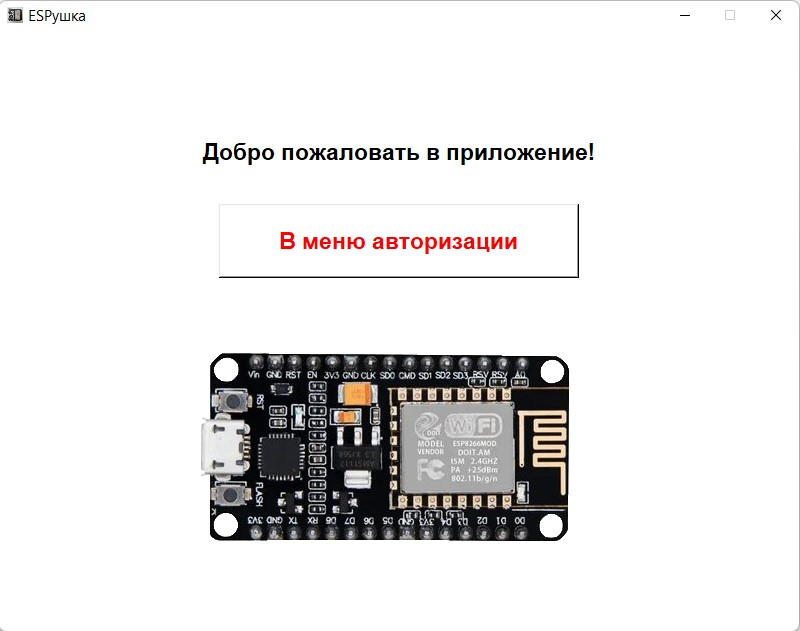
\includegraphics[width=0.5\linewidth]{Pics/WelcomeScreen.jpg}
    \caption{Экран приветсвия.}
    \label{fig:pk1}
\end{figure}

\noindent
После нажатия на кнопку войти пользователь перейдет на экран авторизации(Рис. 2), 
где ему будет предложен выбор войти с учетом имеющегося аккаунта или 
зарегистрироваться(Рис. 3). 

\begin{figure}[htp]
    \centering
    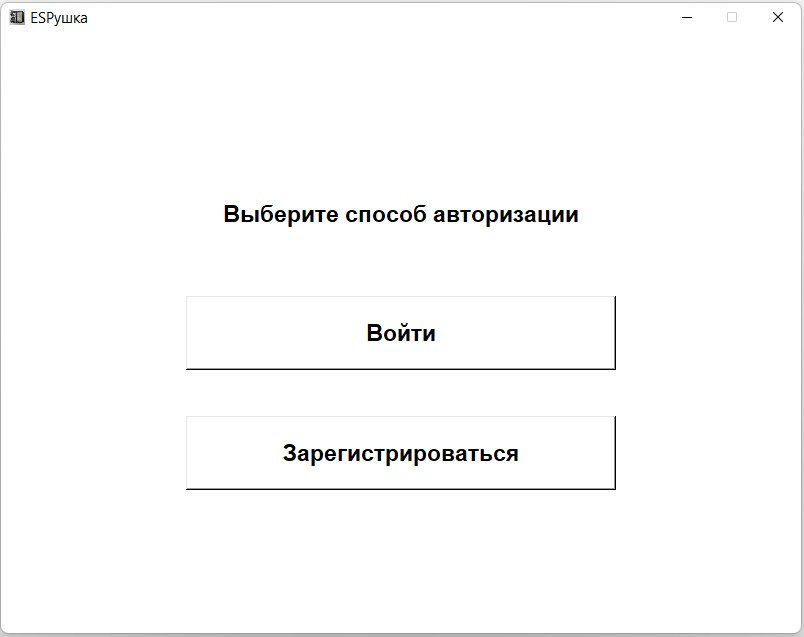
\includegraphics[width=0.5\linewidth]{Pics/AutorizationScreen.jpg}
    \caption{Экран выбора авторизации.}
    \label{fig:pk2}
\end{figure}

\begin{figure}[htp]
  \centering
  \begin{subfigure}[b]{0.5\linewidth}
    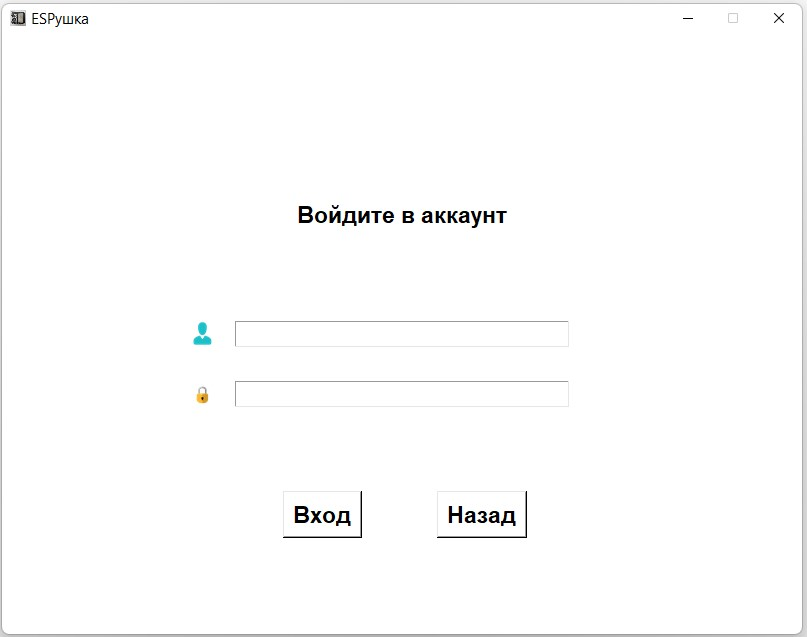
\includegraphics[width=\linewidth]{Pics/SignInScreen.jpg}
    \caption{Экран входа.}
  \end{subfigure}
  \begin{subfigure}[b]{0.5\linewidth}
    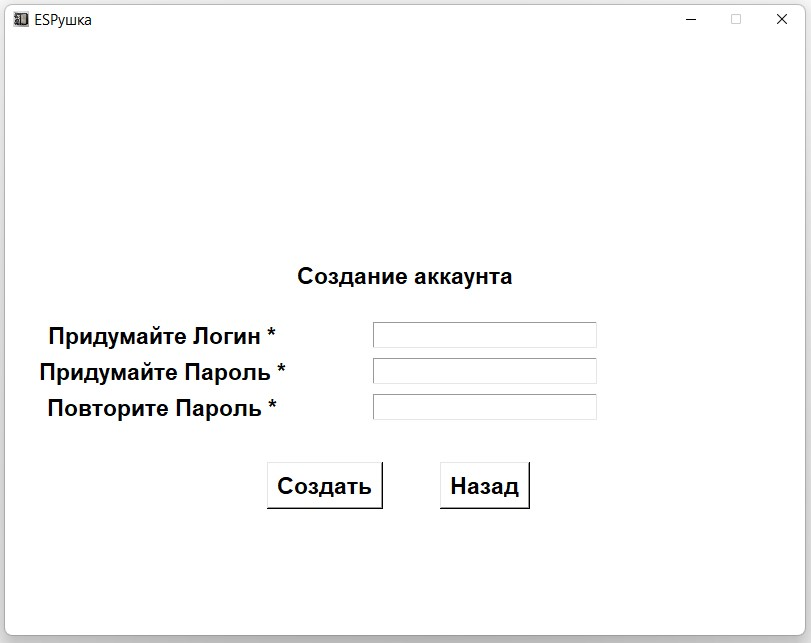
\includegraphics[width=\linewidth]{Pics/SignUpScreen.jpg}
    \caption{Экран регистрации.}
  \end{subfigure}
  \caption{Экран авторизации.}
  \label{fig:pic3}
\end{figure}

\newpage\noindent
После авторизации пользователь попадает на главный экран своего профиля(Рис. 4), где можно перейти на окно просмотра дополнительной информации о своем аккаунте (Рис. 5) или перейти в настройки  и начать подключение к устройству (Рис. 6).

\begin{figure}[htp]
    \centering
    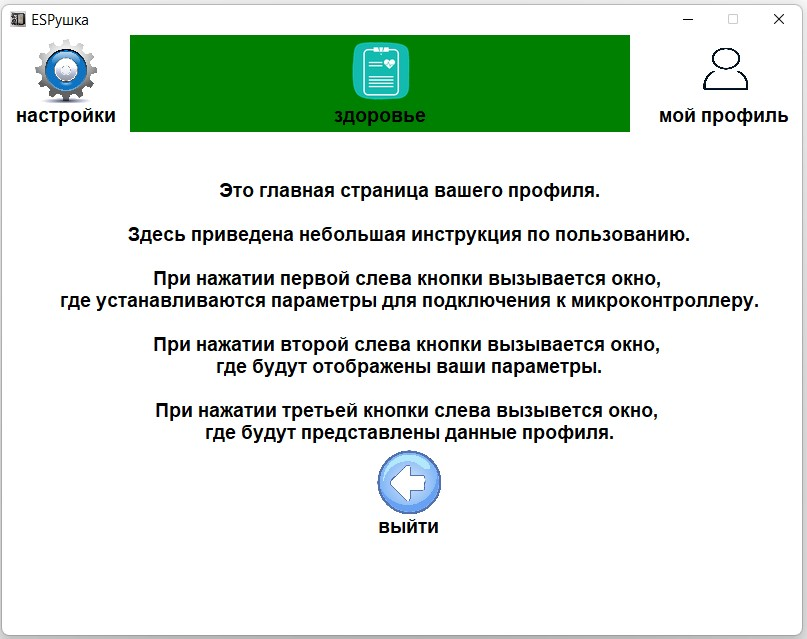
\includegraphics[width=0.6\linewidth]{Pics/ProfileScreen.jpg}
    \caption{Экран главного профиля.}
    \label{fig:pic4}
\end{figure}

\begin{figure}[htp]
    \centering
    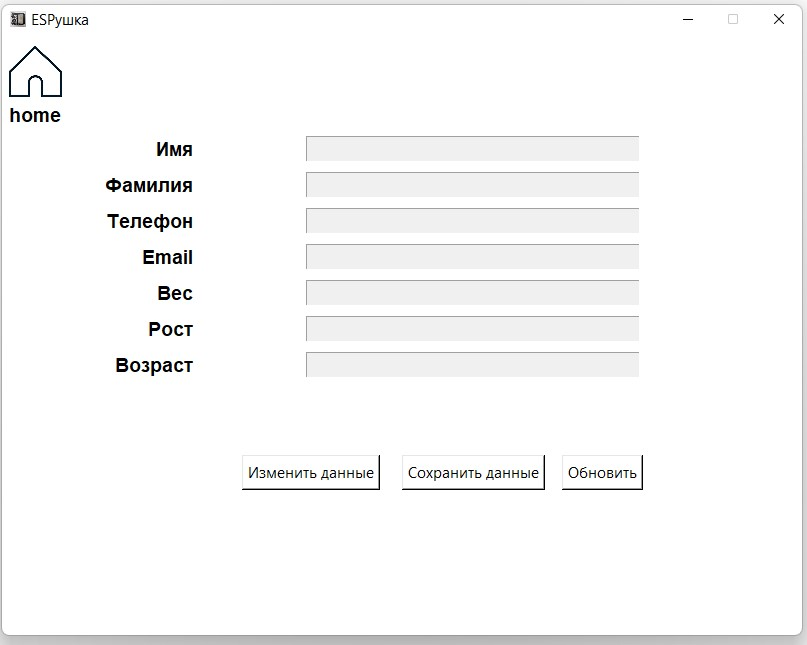
\includegraphics[width=0.5\linewidth]{Pics/AdditionalInfoScreen.jpg}
    \caption{Экран доп. информации.}
    \label{fig:pk2}
\end{figure}

\begin{figure}[htp]
    \centering
    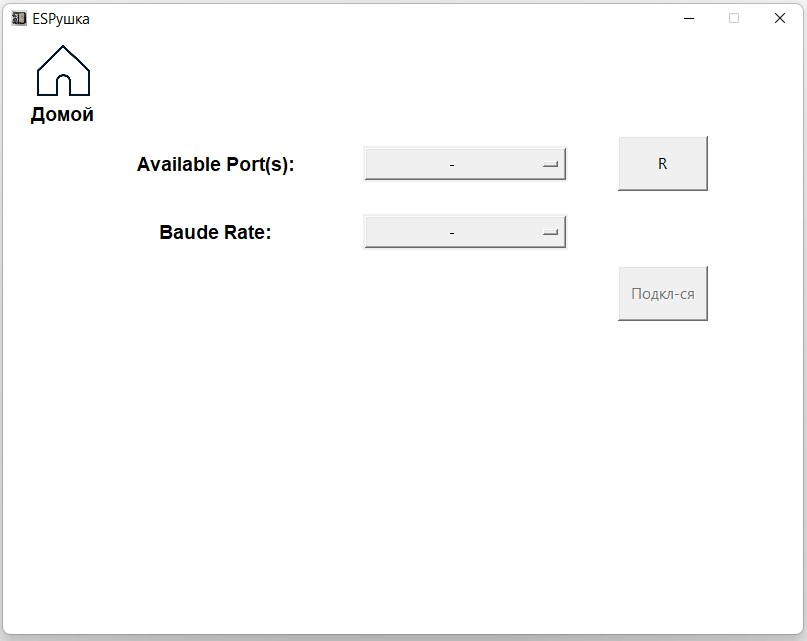
\includegraphics[width=0.5\linewidth]{Pics/SettingsScreen.jpg}
    \caption{Экран настроек.}
    \label{fig:pk2}
\end{figure}

\newpage\noindent
После подключения к устройству, необходимо перейти в окно здоровье, где пользователь может посмотреть график своего пульса или оксигенации (Рис. 7 и 8).

\begin{figure}[htp]
    \centering
    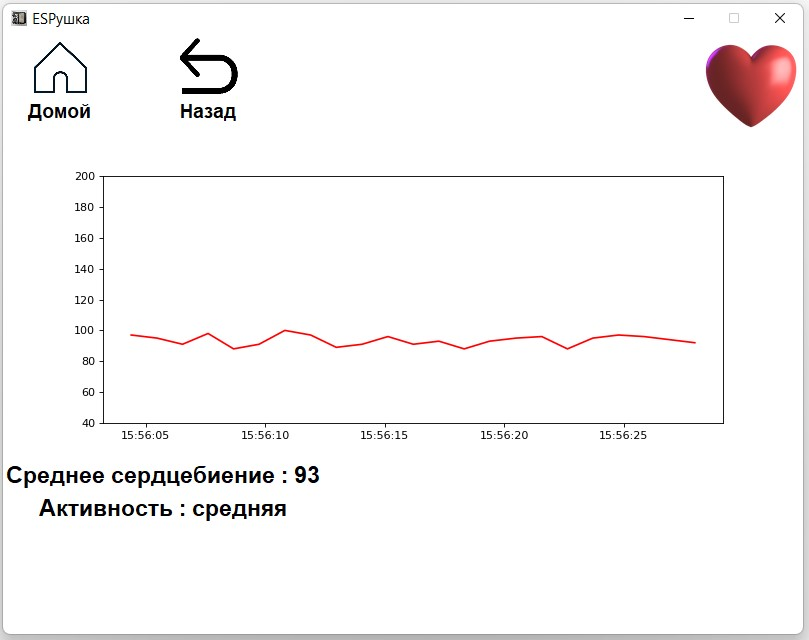
\includegraphics[width=0.5\linewidth]{Pics/BPM.jpg}
    \caption{Экран графика пульса.}
    \label{fig:pk2}
\end{figure}

\begin{figure}[htp]
    \centering
    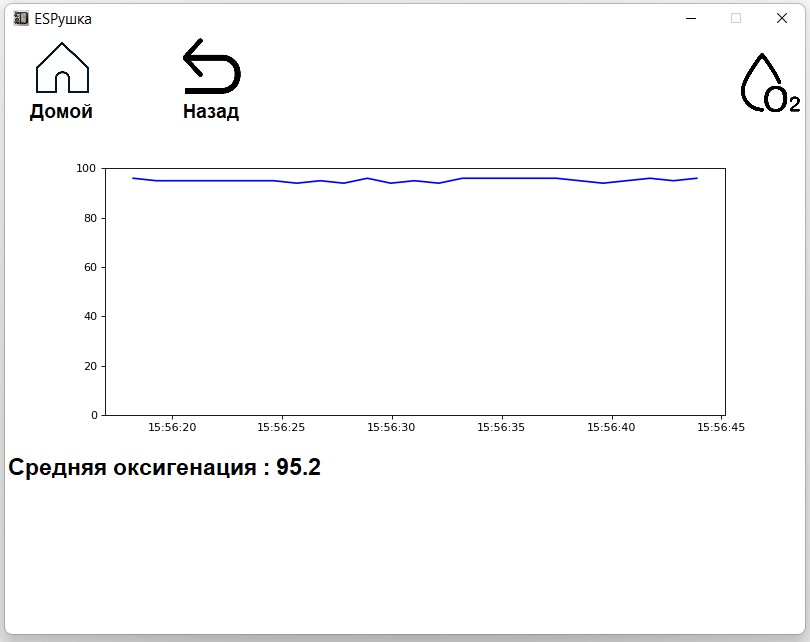
\includegraphics[width=0.5\linewidth]{Pics/SPo2.jpg}
    \caption{Экран графика оксигенации.}
    \label{fig:pk2}
\end{figure}

\newpage
\hfill \break
}

% Заключение (основные результаты)
{


\newpage

\section*{Заключение.} \addcontentsline{toc}{section}{7. Заключение.}

В результате были разработано устройство для регулярного определения состояния здоровья человека. 
В ходе экспериментов были обнаружены недостатки связанные с неточностью датчиков
для измерения, в связи с чем показания прибора могли быть неточными.
\par\noindent
Также нами была написана программа, которая принимает полученные данные и анализирует
их с помощью модели машинного обучения. Полученные показания визуализируются с помощью удобного 
для восприятия графического программного интерфейса.
}

% Список литературы
{


\section*{} \addcontentsline{toc}{section}{8. Список литературы.}
\newpage
\begin{thebibliography}{7}
\bibitem  "Документация к фреймворку TKinter https://docs.python.org/3/library/tkinter.html
\bibitem '"ESP32 Datasheet" (PDF). Espressif Systems. 2017-03-06. Retrieved 2017-03-14.
\bibitem '"Microcontroller Maniacs Rejoice: Arduino Finally Releases the 32-Bit Due". Wired. Retrieved 20 February 2018.
\bibitem '"Getting Started: FOUNDATION > Introduction". arduino.cc. Archived from the original on 2017-08-29. Retrieved 2017-05-23.
\bibitem 'J. M. Hughes: Arduino: A Technical Reference. O'Reilly Media, 2016, ISBN 978-1-4919-3450-0, S. 122 ff.
\bibitem 'McKinney, Wes (2017). Python for Data Analysis : Data Wrangling with Pandas, NumPy, and IPython (2nd ed.). Sebastopol: O'Reilly. ISBN 978-1-4919-5766-0.
\bibitem 'VanderPlas, Jake (2016). "Introduction to NumPy". Python Data Science Handbook: Essential Tools for Working with Data. O'Reilly. pp. 33–96. ISBN 978-1-4919-1205-8.
\end{thebibliography}

}

% Приложения (если есть)
{
\newpage

\section*{Приложения.} \addcontentsline{toc}{section}{9. Приложения.}
Код приложения находится в репозитории : 
\\ https://github.com/danielbulgakov/ITlab\_Project
}



\end{document}